\chapter{Project implementation}
The project is developed in Pandapower a, Python based, power system analysis tool aimed at automation of static and quasi-static analysis and optimization of balanced power systems \cite{pandapower}.

\section{GYM-ANM}
The network employed for these experiments is the network used in the paper \cite{gym-anm}; it consists of: one external grid, five buses, one transformer, four lines, three loads, two static generators and one \gls{DES} device.

\begin{figure}[h]
\centering
    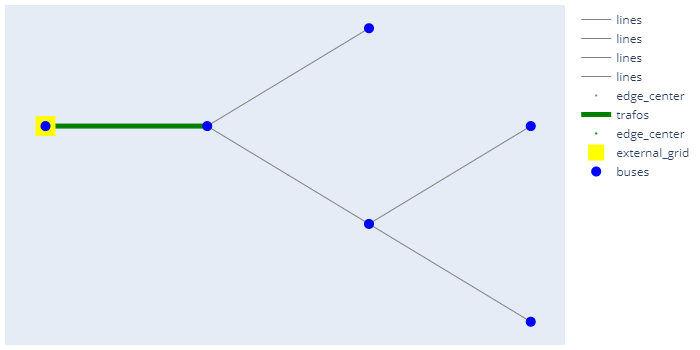
\includegraphics[width=.7\linewidth]{images/GYM-ANM/NETS/Gyn-anm network.png}
\caption{GYM-ANM network}
\label{fig:gym_anm_net}
\end{figure}

\noindent Following the paper, 3 situations are tested obtaining similar results:\\
\textbf{Situation 1} \\
    This situation (figure: \ref{fig:net_sit1}) characterises a windy night, when the consumption is low, the PV
    production null, and the wind production at it is near maximum. Due to the very low demand from the industrial load, the wind production must be curtailed to avoid an overheating of the transmission lines connecting
    buses 0 and 4.
    \begin{figure}[H]
    \centering
        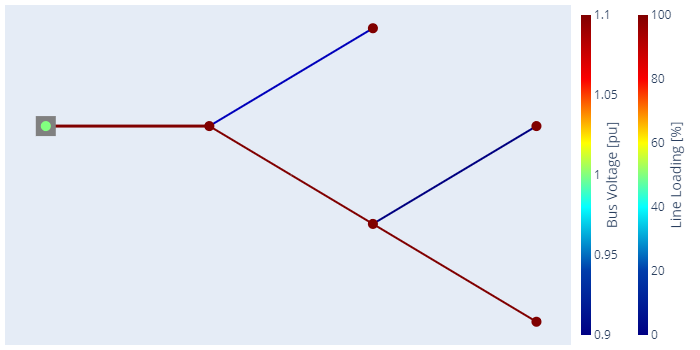
\includegraphics[width=.7\linewidth]{images/GYM-ANM/NETS/Gyn-anm network situation1.png}
    \caption[GYM-ANM network situation 1]{GYM-ANM network situation 1. Interactive image at the following \href{https://htmlpreview.github.io/?https://github.com/MauriVass/ThesisLiege/blob/master/Images/fig_case1.html}{link}}
    \label{fig:net_sit1}
    \end{figure}
    
\noindent \textbf{Situation 2} \\
    In this situation (figure: \ref{fig:net_sit2}), bus 5 is experiencing a substantial demand due to a large number
    of EVs being plugged-in at around the same time. This could happen in a large public EV charging garage. In the morning, workers of close-by companies would plug in their car after arriving at work and, in the evening, residents of the area would plug in their cars after getting home. In order to emphasise the problems arising from this large, localised demand, we assume that the other buses (3 and 4) inject or withdraw very little power into/from the network. During those periods of the day, the DES unit must provide enough power to ensure that the transmission path from bus 0 to bus 5 is not overrated, which would lead to an overheating of the line. For this to be possible, the agent must strategically plan ahead to ensure a sufficient charge level
    at the \gls{DES} unit.
    \begin{figure}[h]
    \centering
        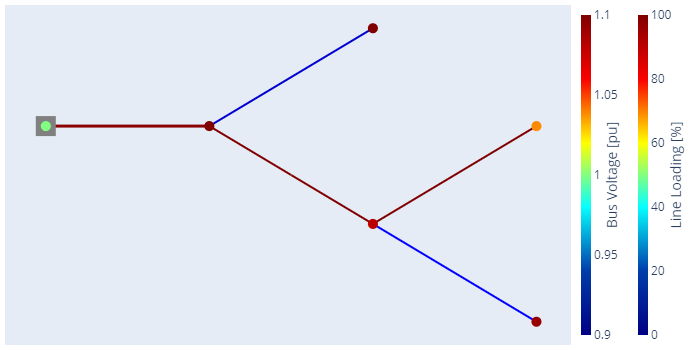
\includegraphics[width=.7\linewidth]{images/GYM-ANM/NETS/Gyn-anm network situation2.png}
    \caption[GYM-ANM network situation 2]{GYM-ANM network situation 2. Interactive image at the following \href{https://htmlpreview.github.io/?https://github.com/MauriVass/ThesisLiege/blob/master/Images/fig_case2.html}{link}}
    \label{fig:net_sit2}
    \end{figure}
    
\noindent \textbf{Situation 3} \\
    Situation (figure: \ref{fig:net_sit3}), represents a scenario that might occur in the middle of a sunny windy weekday. No one is home to consume the solar energy produced by residential PVs at bus 1 and the wind energy production exceeds the industrial demand at bus 2. In this case, both renewable generators should be
    adequately curtailed while again storing some extra energy to anticipate the EV late afternoon charging period, as depicted in Situation 2.
    \begin{figure}[h]
    \centering
        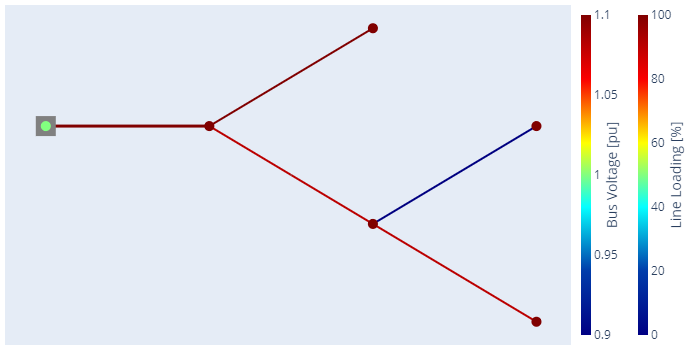
\includegraphics[width=.7\linewidth]{images/GYM-ANM/NETS/Gyn-anm network situation3.png}
    \caption[GYM-ANM network situation 3]{GYM-ANM network situation 3. Interactive image at the following \href{https://htmlpreview.github.io/?https://github.com/MauriVass/ThesisLiege/blob/master/Images/fig_case3.html}{link}}
    \label{fig:net_sit3}
    \end{figure}
    
\subsection{Generate dataset}
Pandapower allows running time series simulations of a network. When calling the time series function, a loop starts to iterate for each time step and the power flow of the network is calculated.\\
For this simulation, a time $\Delta t$ of 15 minutes if used for a temporal window of one year, in total of 35,040 time steps. To be compliant to Pandapower requirements, the time series must be passed to a controller that will change the network's devices values for each loop.\\
The results in this section are obtained with the following time series:

\begin{algorithm}[H]
\caption{Time series of active power \gls{P} for loads \gls{L} and generators \gls{G}}
\label{alg:timeseries}
\begin{algorithmic}[1]
\State $n\_timesteps = 365 * 24 * 4$

\LineComment{Loads active power}
\State $Load0\_p = cos(range(n\_timesteps))^2* rand(n\_timesteps)*4$
\State $Load1\_p = normal(7,0.5, size=n\_timesteps)$
\State $Load2\_p = normal(14,0.5, size=n\_timesteps)$

\LineComment{Generators active power}
\State $PVgen\_p = normal(4,0.5, size=n\_timesteps)$
\State $Windgen\_p = cos(range(n\_timesteps))^2*rand(n\_timesteps)*12$

%\end{small}
\end{algorithmic}
\end{algorithm}

After the simulation is run, some output values are exported as \emph{.xlsx} files and these constitute the dataset, the story of the network. These output values are:
\begin{itemize}
    \item loads active power in MW.
    \item buses voltage magnitude in \gls{pu}.
    \item the lines loading in percentages and the current in kA.
\end{itemize}

\begin{figure}[h]
    \centering
    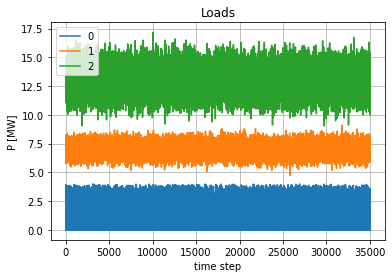
\includegraphics[width=.32\linewidth]{images/GYM-ANM/DATASET PLOTS/loads.png}
    \includegraphics[width=.32\linewidth]{images/GYM-ANM/DATASET PLOTS/VM.png}
    \includegraphics[width=.32\linewidth]{images/GYM-ANM/DATASET PLOTS/LL.png}
    \caption[GYM-ANM datasets]{Loads active power, buses voltage magnitude and line percentage loading}
    \label{fig:net_sit3}
\end{figure}
    
    
\subsection{Voltage lines forecasting}
\subsubsection{Splitting the dataset}
The aforementioned dataset is divided in training, validation and test set in 70, 20 and 10 percent respectively, without a random shuffle before the splitting. This has two main advantages:
\begin{enumerate}
    \item It ensures that chopping the data into windows of consecutive samples is still possible.
    \item It ensures that the validation/test results are more realistic, being evaluated on the data collected after the model was trained.
\end{enumerate}

\subsubsection{Normalization}
The data is normalised subtracting the mean and dividing by the standard deviation of each feature. The mean and standard deviation are computed using the training data so that the models have no access to the values in the validation and test sets.

\subsubsection{Windowing}
The training, validation and test sets are divided in windows to then fed to the neural network. \\
The main features of the windows are:
\begin{itemize}
    \item The width (number of time steps) of the input and label windows.
    \item The time offset between them.
    \item Which features are used as inputs, labels, or both.
\end{itemize}

The result are obtained using an input window of 12 time steps (3 hours in the past) and an output window of 6 time steps (1.5 hours in the future). The offset is 1, this means that the predictions are from time step 13 to 18. The training features are:
\begin{algorithmic}
\State $[load0\_p, load1\_p, load2\_p, PVgen\_p, Wind gen\_p, L0, L1, L2, L3]$
\end{algorithmic}
and the label features are:
\begin{algorithmic}
\State $[L0, L1, L2, L3]$
\end{algorithmic}
where $Li$ is the loading in percentage of line $i$.

\begin{figure}[h]
    \centering
    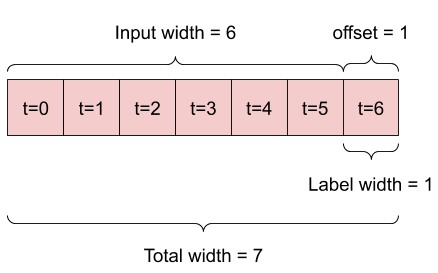
\includegraphics[width=.7\linewidth]{images/GYM-ANM/DATASET PLOTS/raw_window_1h.png}
    \caption[GYM-ANM datasets windowing]{Window visual representation for the input and output time steps \\
    TODO: add an image that shows the real situation (This is taken from Tensorflow website)}
    \label{fig:net_sit3}
\end{figure}

\subsubsection{Training}
The model used for training is an artificial neural network with two hidden layers with 128 and 64 neurons respectively.\\
The neural network is trained for 20 epochs with Adam optimizer and early stopping callback.

\begin{figure}[H]
    \centering
    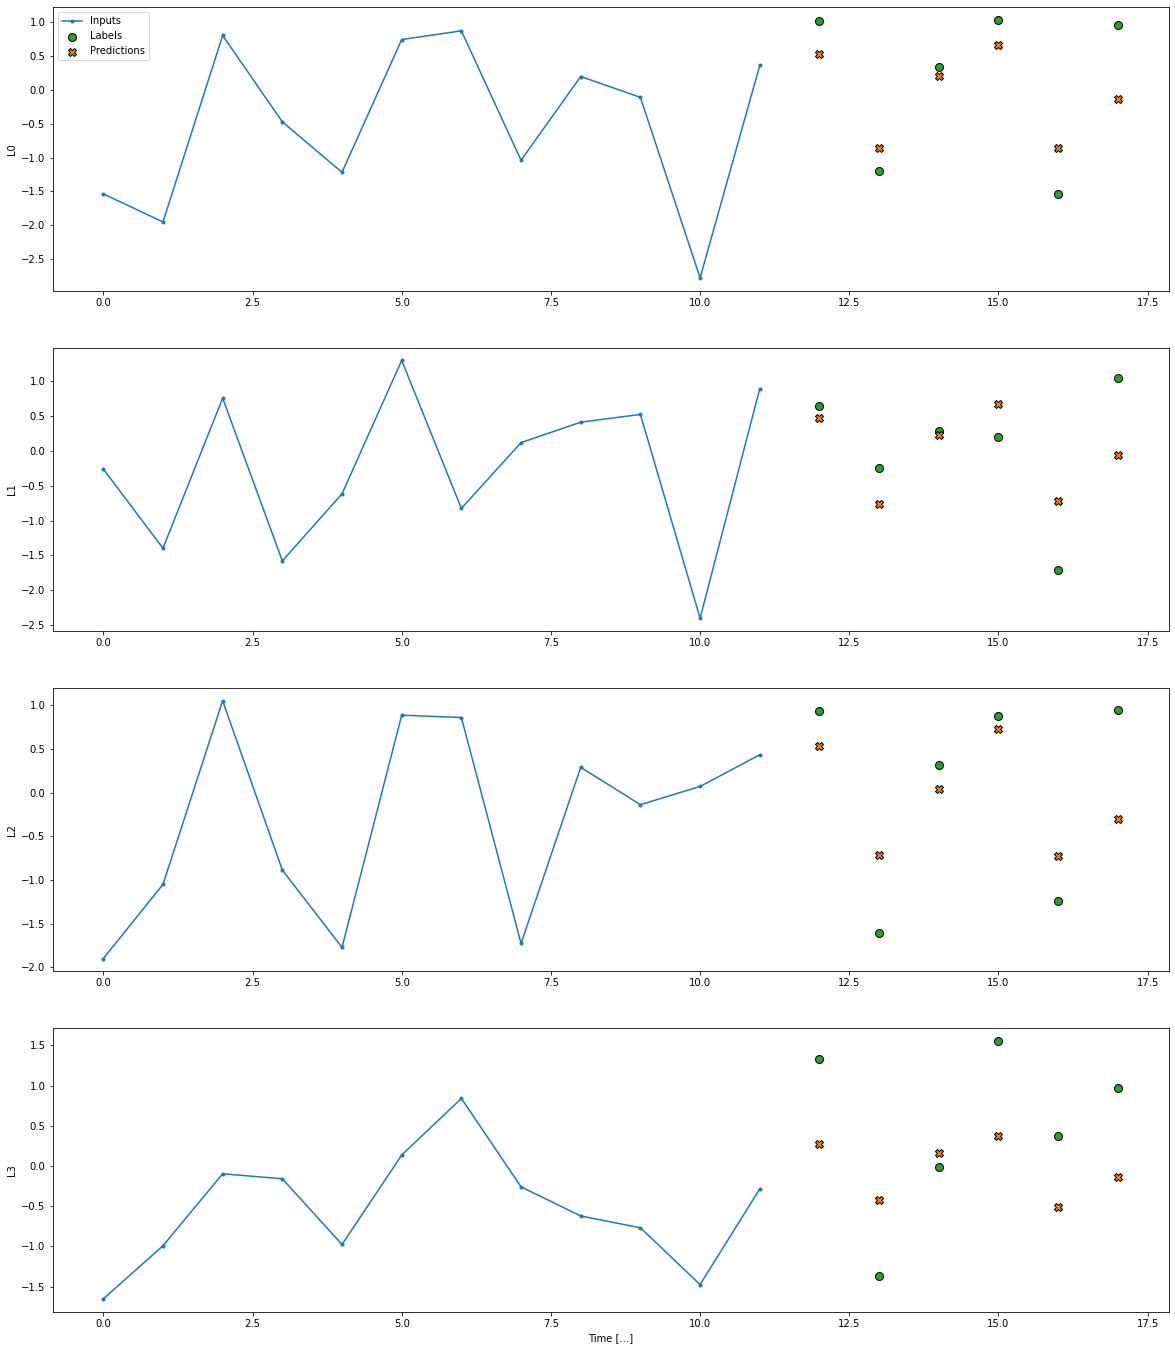
\includegraphics[width=.5\linewidth]{images/GYM-ANM/DATASET PLOTS/lines_forecasting.png}
    \caption[GYM-ANM forecasting]{Forecasting of the values \\
    TODO: denormalise the data for visualisation purposes. Decrease height or split it: too large for this template (it messes up with the layout)}
    \label{fig:net_sit3}
\end{figure}

\noindent The metric used for the evaluation is the mean absolute error (\gls{MAE}):
\begin{algorithmic}
\State $mean\_absolute\_error: 0.6201$
\LineComment{MAE for each feature}
\State $\{L0:0.5625071, L1:0.613873 , L2:0.5569194, L3:0.7471818]$
\end{algorithmic}

\noindent Given this voltage forecast, it would be possible to understand if the network risks overloading for the next time steps and proceed accordingly to avoid damaging the network.



\section{MV Oberrhein}
\label{sec:MVober}
The network used for these experiments is the MV Oberrhein network from Pandapower; a generic 20 kV network serviced by two 25 MVA HV/MV transformer stations. The network supplies 141 HV/MV substations and 6 MV loads through four MV feeders. The network layout is meshed, but the network is operated as a radial network with 6 open sectioning points. \\
To simplify the situation, the network can be divided in 2 independent parts [\href{https://kobra.uni-kassel.de/bitstream/handle/123456789/12005/kup_9783737608725.pdf?sequence=1&isAllowed=y}{ref}].

\begin{figure}[h]
\centering
    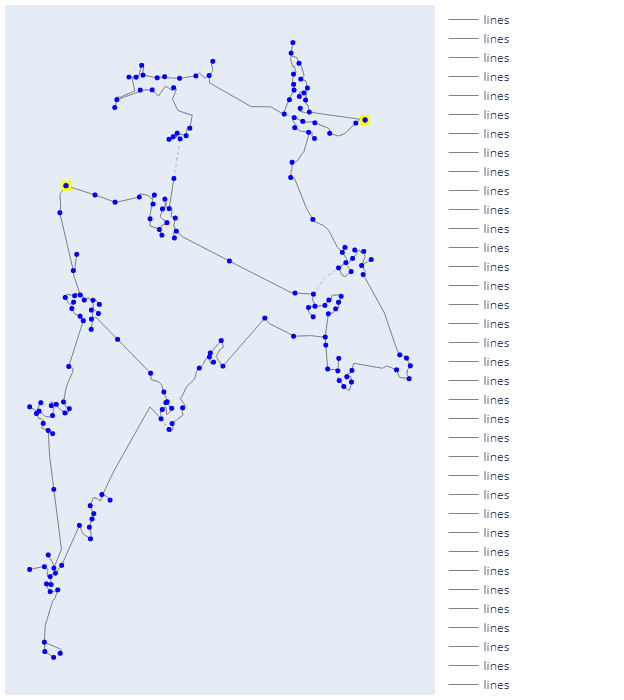
\includegraphics[height=0.33\linewidth,width=.32\linewidth]{images/MVOberr/Full.png}
    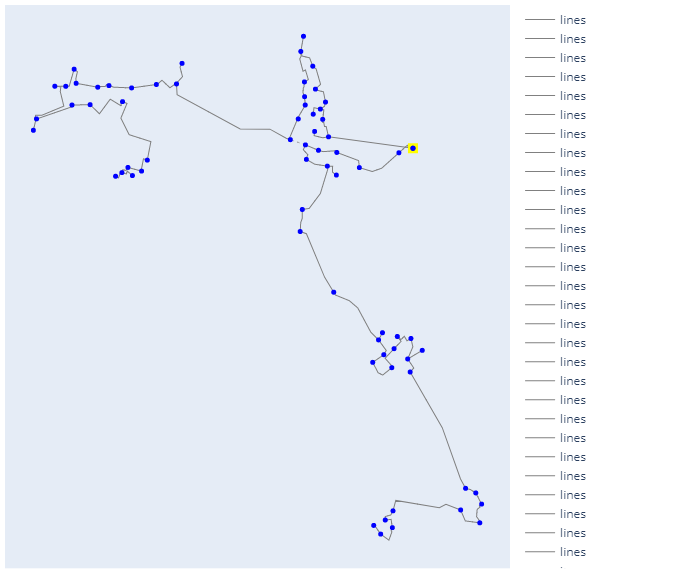
\includegraphics[height=0.33\linewidth,width=.32\linewidth]{images/MVOberr/Half1.png}
    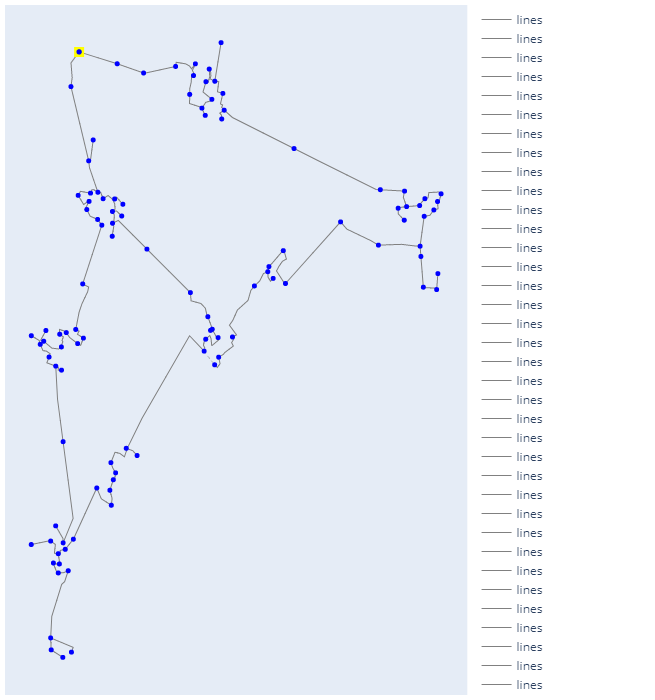
\includegraphics[height=0.33\linewidth,width=.32\linewidth]{images/MVOberr/Half2.png}
\caption{MV Oberrhein network. Used network: middle one \\
TODO add letters}
\label{fig:gym_anm_net}
\end{figure}

The model consist of: one external grid, one transformer, 70 buses, 61 loads and 60 renewable generators.

\subsection{Simbench database}
\label{simdata}
\emph{Q: Better to move it to the 'Background' chapter?}\\
The time series dataset used is taken from the Simbench database. This database refers to some real distribution networks in Germany in the year 2016. SimBench includes multiple time series for one year with 15 min resolution for load, generation and storage units. All time series came as active and reactive power. The time series were normalized, reducing the total number of required time series to a reasonable number, while retaining the possibility to model individual nominal power \cite{Simbenchds0}. All active power values are normalized to the maximum active power value.\\

Power utilities commonly use generic load profiles to group commercial customers with similar load shapes into categories or standard load profiles (\glspl{SLP}). \\
The most commonly used profiles set is developed by the German Association of Energy and Water Industries (BDEW). It comprises eleven aggregated profiles, one for residential consumers (H0), three for agricultural (L0-L3), and seven for commercial consumers with different opening hours (G0-G6). They are differentiated into workdays, Saturdays and Sundays as well as three seasonal categories winter, summer, and transitional. The set also includes two profiles for street lightning (B0) and band load (G7). \\
The generation time series for photovoltaics (\glspl{PV}), wind energy and biomass generated for the SimBench dataset are created using the agent-based simulation tool for optimized grid expansion planning SIMONA. SIMONA's power plant models receive real weather data of Germany from the German Weather Service in 2011 for Wind and 2012 for \gls{PV} time series as input data. \\
For 2011 and 2012 generation data, the time axis is adjusted to 2016 by shifting days so that they correspond to the nearest weekday\cite{Simbenchds1}.\\

\begin{figure}[h]
\centering
    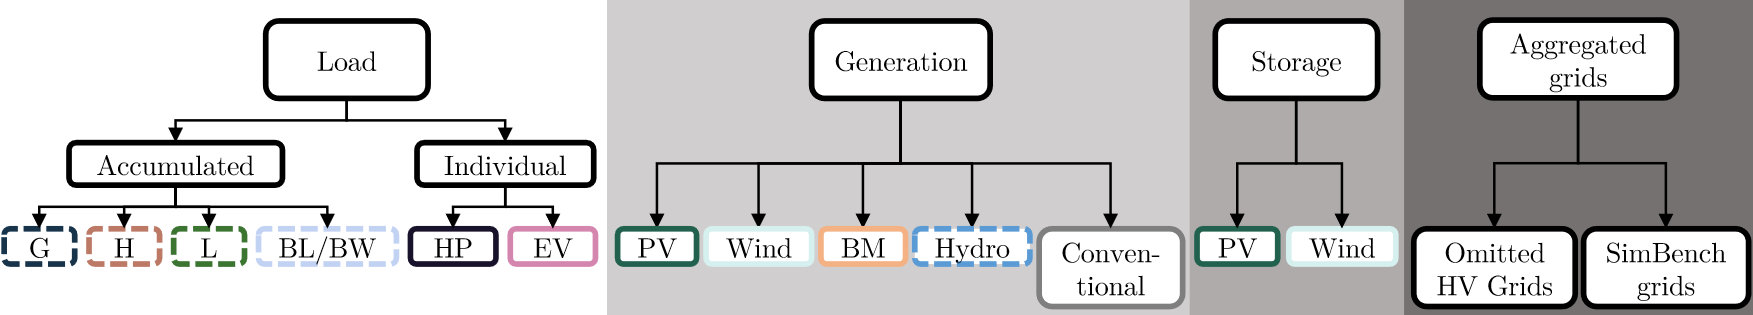
\includegraphics[width=.8\linewidth]{images/MVOberr/SimBench time series types.PNG}
\caption{Overview of the SimBench time series type}
\label{fig:SBtimeseriestype}
\end{figure}

The load time series were distinguished between real measured accumulated, highlighted with a dash, and simulated individual consumers, marked with a solid frame in Figure \ref{fig:SBtimeseriestype}. \\

\subsection{Time series}
\label{ts}
Some time series from the Simbench database are taken to adapt to the number of loads and \glspl{DER} of the MV Oberrhein network in consideration. \\

As said, each element (load or generator) falls under a specific profile type that represent the consumption or generation over time.

\begin{figure}[H]
\centering
    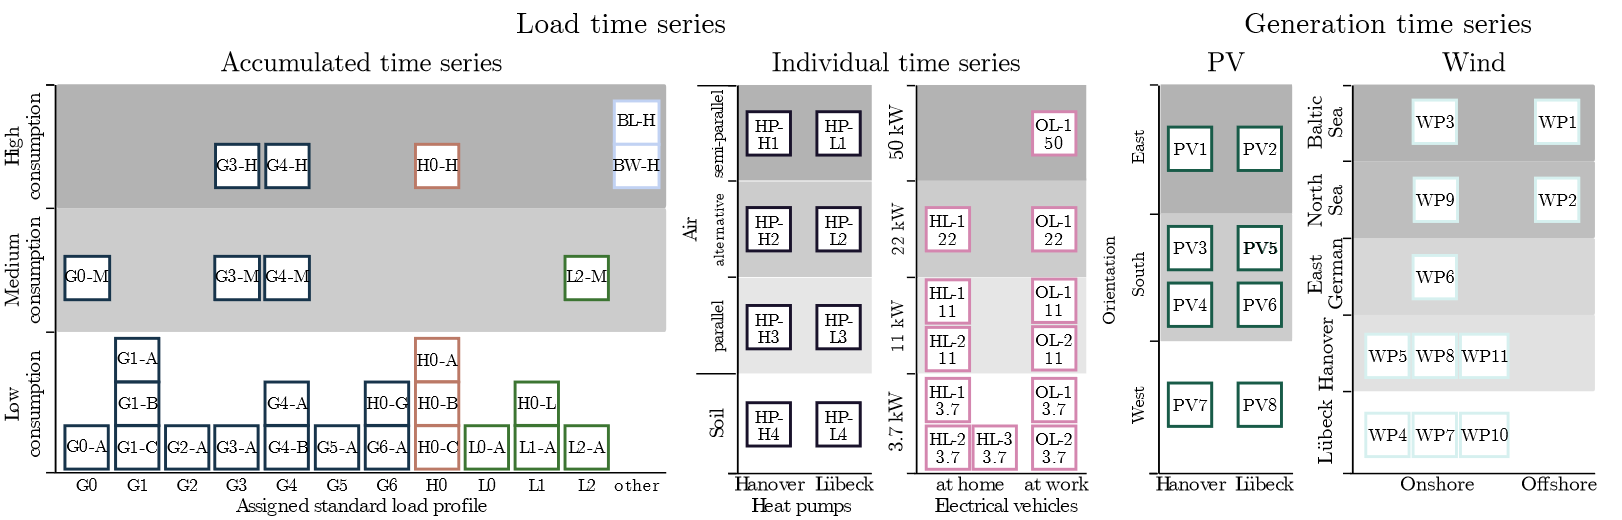
\includegraphics[width=.8\linewidth]{images/MVOberr/SimBench load and generation time series.PNG}
\caption{Load and generations profiles}
\label{fig:gym_anm_net}
\end{figure}

In this case, the profiles' distribution in the Pandapower network is as follows:

\begin{algorithm}[h]
\State Load elements by type: \{'L2-A': 24, 'H0-C': 5, 'L1-A': 23, 'H0-B': 5, 'H0-A': 4\}

\State{RES elements by type: \{'PV5': 27, 'PV8': 14, 'PV6': 13, 'WP4': 3, 'WP7': 3\}}
\end{algorithm}
\noindent where the letters stand for: commercial enterprises (G), households (H), agricultural holdings (L) and industrial companies (BL/BW)'; with last letters –A to C indicating low consumption, -M medium consumption, and -H high consumption customers. \\
For the \gsl{DES} device there are photovoltaics \glspl{PV} and wind parks \glspl{WP}. It is possible to notice a bigger presence of \glspl{PV} over \glspl{WP}.\\

The loads and \glspl{DER} are chosen so that different profile types are present.



\begin{figure}[H]
\centering
    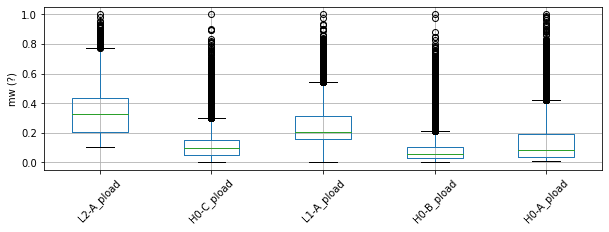
\includegraphics[width=.7\linewidth]{images/MVOberr/BoxPlotLoad.png}
    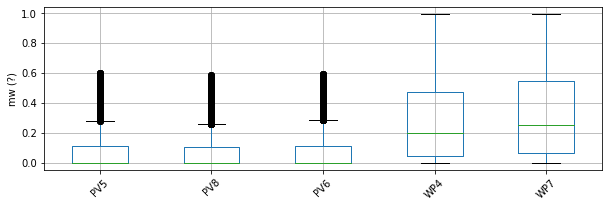
\includegraphics[width=.7\linewidth]{images/MVOberr/BoxPlotRes.png}
\caption{Box plots of load and generation for each profile type}
\label{fig:gym_anm_net}
\end{figure}

\emph{Q: Is it ok that elements of the same type have the same profile, so same consumption/generation over time? R: add some noise} \\
\emph{Q: Also from the documentation the values of the profiles are in MW, but it looks strange that the values never go above 1MW, is it common that facilities (small or big) consumes less than a 1MW? R: it depends on the device. Actually, the values are normalized, so a scaling factor can be used to change the values.} \\

Since the profiles are equal for every element of that type, some noise is added to increase randomness. In particular, the noise added is a scaling factor in the range [0.85,1.15]. The scaling factor allows avoiding negative values in case of a value lower than 1; subtraction may result in a negative value of reactive power for a particular load. \\

With a similar approach, it is possible to easily create different cases, changing the scaling factors.

\begin{figure}[H]
\centering
    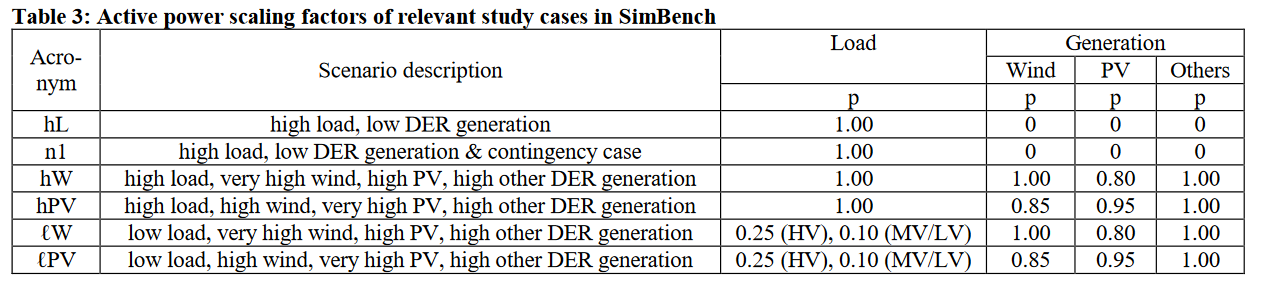
\includegraphics[width=.9\linewidth]{images/MVOberr/Cases.PNG}
\caption{Possible cases. [\href{https://www.cired-repository.org/bitstream/handle/20.500.12455/526/CIRED \%202019 \%20- \%20139.pdf?sequence=1&isAllowed=y}{ref}] }
\label{fig:gym_anm_net}
\end{figure} 



\begin{figure}[h]
\centering
    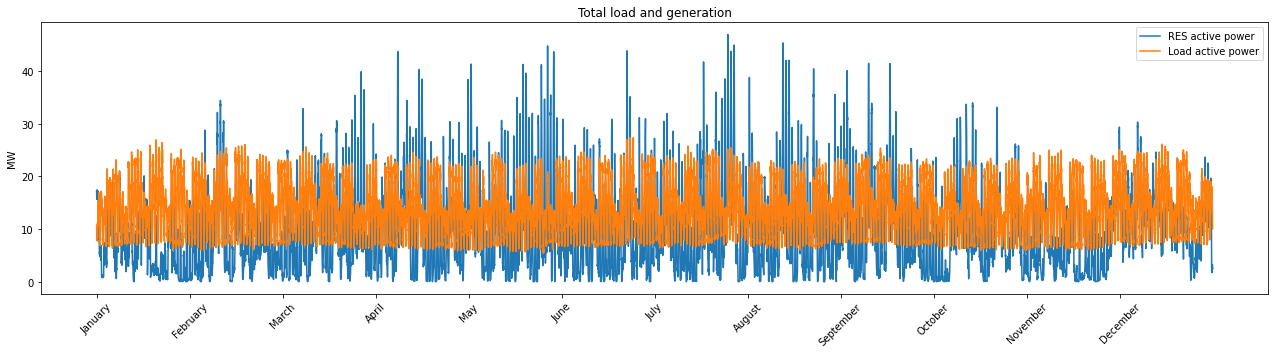
\includegraphics[width=.9\linewidth]{images/MVOberr/Load&Gens.png}
\caption{Sum of load energy consumption and energy generation over the considered year}
\label{fig:gym_anm_net}
\end{figure}

It is possible to notice a higher consumption of energy over the production, especially at the beginning and end of the year, when the sun intensity is not too high. \\

\subsubsection{Case: High generation}
Some cases are tested using scaling factors for load and generation. The high resolution case refers to scaling factors, as follows:
\begin{algorithm}[h]
    \State {scale\_factor\_load = 0.5} 
    
    \State {scale\_factor\_sgen = 3.5}
\end{algorithm}

\begin{figure}[H]
\centering
    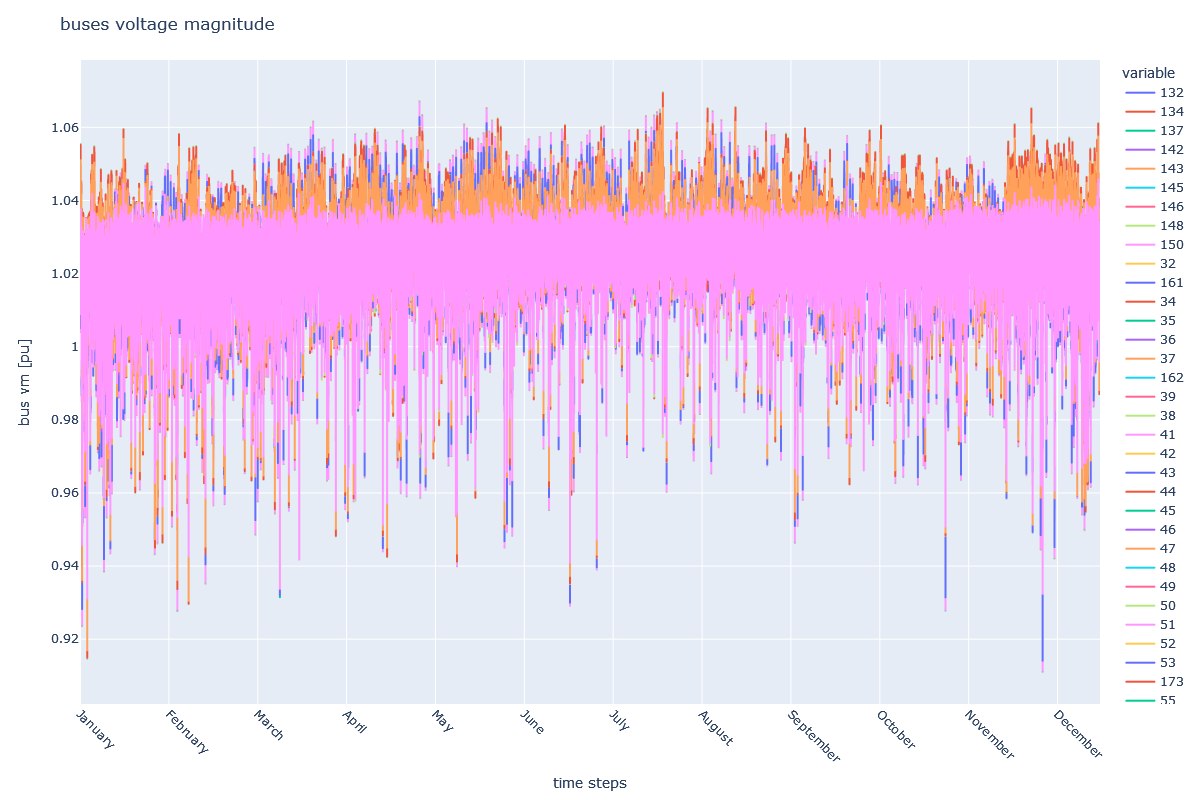
\includegraphics[width=.7\linewidth]{images/MVOberr/High gen.png}
\caption{Case high generation. Voltage buses results obtained running the time series. \emph{For a faster execution, only 7 days (672 time steps) are considered. Time step 0 correspond to 00:00 of 01/01/2016.}}
\label{fig:gym_anm_net}
\end{figure}

From the plot above, it is possible to see that there are few overvoltage problems and many under voltage problems. A time step is critical when the voltage of any bus is out of the boundaries $V_i < v^{\text{min}}$ (under voltage) or $V_i > v^{\text{max}}$ (over voltage), where $v^{\text{min}}$ is the minimum acceptable voltage, 0.95, and $v^{\text{max}}$ is the maximum one, 1.05. \\
The problems are highlighted in the following plot.

\begin{figure}[H]
\centering
    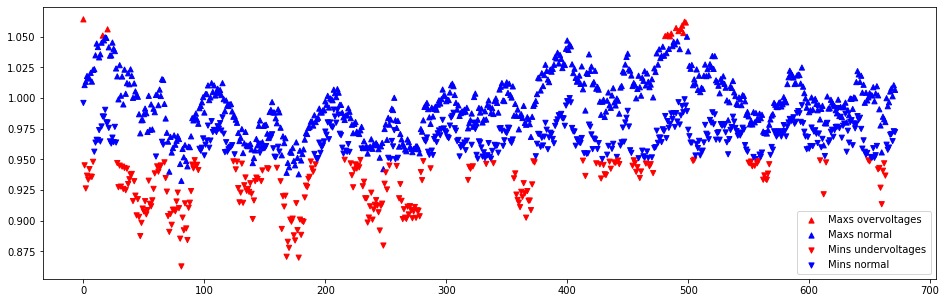
\includegraphics[width=.8\linewidth]{images/MVOberr/High gen problems.png}
\caption{In this plot, the maximum and minimum values found for each time step and plotted, so for each time step there are two values representing the highest and lowest value among each bus. The colours, blue and red, represent the normal or critical condition}

 \end{figure}






\subsubsection{Case: High load}
The high load case refers to scaling factors, as follows:
\begin{algorithm}[h]
    \State {scale\_factor\_load = 1} 
    
    \State {scale\_factor\_sgen = 0.1}
\end{algorithm}

\begin{figure}[h]
\centering
    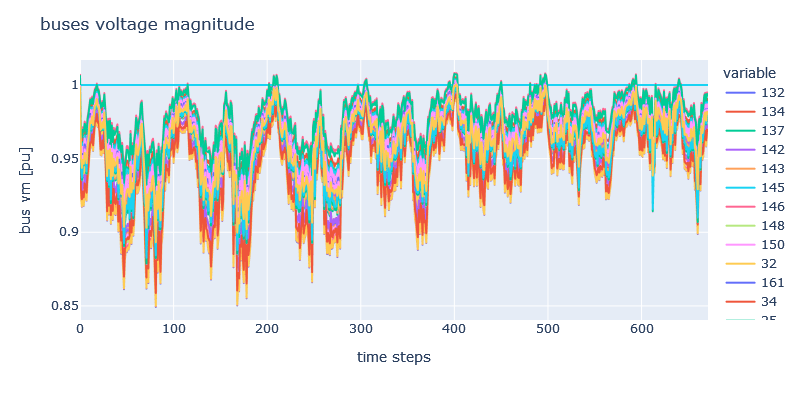
\includegraphics[width=.7\linewidth]{images/MVOberr/High load.png}
\caption{Case high load. Voltage buses results obtained running the time series}
\label{fig:gym_anm_net}
\end{figure}

In this case, there are only under voltage problems. \\
The problems are highlighted in the following plot.

\begin{figure}[h]
\centering
    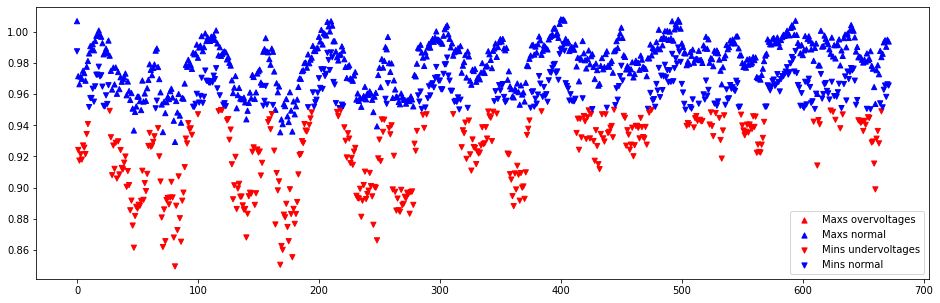
\includegraphics[width=.8\linewidth]{images/MVOberr/High load problems.png}
    \caption{Same as above, the maximum and minimum values found for each time step and plotted, so for each time step there are two values representing the highest and lowest value among each bus. The colours, blue and red, represent the normal or problem condition.}
\end{figure}